\documentclass[parskip=full]{scrartcl}
\usepackage[utf8]{inputenc} % use utf8 file encoding for TeX sources
\usepackage[T1]{fontenc}    % avoid garbled Unicode text in pdf
\usepackage[german]{babel}  % german hyphenation, quotes, etc
\usepackage{hyperref}       % detailed hyperlink/pdf configuration
\usepackage{graphicx}       % provides commands for including figures
\usepackage{csquotes}       % provides \enquote{} macro for "quotes"
\usepackage[nonumberlist]{glossaries}     % provides glossary commands
\usepackage{enumitem}
\usepackage{setspace}
\usepackage{subfigure}
\usepackage{pgf}

\makenoidxglossaries

\newglossaryentry{nn}
{
	name={neural network},
	description={a network or a circuit of neuron used for information processing inspired by the way biological neural systems process data},
	plural=neural networks
}

\newglossaryentry{img}
{
	name={image},
	description={a two dimensional matrix of red,green,glue (RGB) values that can be visualized as each cell represents a single pixel on the monitor. (ex.: a photo)},
	plural=images
}

\title{Specifications}
\author{}
\begin{document}

\maketitle

\section{Preface}

\section{Goal}
The goal is a software which performs image classification and is able to switch between deploy platforms and working modes.
It also should have a GUI to control the software and to show the results.

\section{Product use}
Image classification

\section{Acceptance criteria}
\subsection{Must}
\begin{tabular}{p{2cm}p{12cm}}
\textbf{AC30} & \textbf{Different operating modes} \\
& The software has three modes. One mode for high perfomance, one for low power consumption and one for high energy effiency. \\
\textbf{AC50} & \textbf{Performance and power consumption prediction}\\
& The software can predict the performance with a certain powerconsumption an also the powerconsumption for a certain performance.
\end{tabular}
\begin{itemize}[nosep]
\item [MAC010]: Image classification
\item [MAC020]: Running NN on heterogenous platforms, CPU and FPGA
\item [MAC030]: Different operating modes
\item [MAC040]: GUI for interacting with software
\item [MAC050]: Performance/power prediction
\end{itemize}

\subsection{Can}
\begin{itemize}[nosep]
\item [KAC060]: Training a nn for classification
\item [KAC070]: Illustration of a topology of the nn
\item [KAC080]: Object detection
\item [KAC090]: Choosing between different models
\item [KAC100]: Creating new models
\item [KAC110]: Voting of multiple nn
\item [KAC120]: Using video for classification
\item [KAC130]: Using camera for classification input
\item [KAC140]: Running NN on GPU
\end{itemize}

\section{Functional Requirements Must}
\begin{itemize}[nosep]
\item [MFR025]: Dispatching the calculation process defined from the mode
\item [MFR030]: Support CPU for calculation
\item [MFR031]: Support FPGA for calculation
\item [MFR040]: Communication between Host-PC and platform
\item [MFR041]: Send image for classification
\item [MFR042]: Receive result
\item [MFR050]: GUI
\item [MFR060]: Showing results
\end{itemize}
\begin{tabular}{p{2cm}p{12cm}}

\textbf{MFR010} & \textbf{Use \gls{nn} for \gls{img} classification}\\                                     
& A \gls{nn} should be used in order to classify \glspl{img} based on what is shown on them. For each \gls{img} a list of possible classes it could belong to along with degree of confidence should be given as output.\\
& \\
\textbf{MFR011} & \textbf{Deploy pre-trained \gls{nn} with the corresponding layers}\\
& A pre-trained \gls{nn} should be deployed to with all the corresponding layers in order to fulfill MFR010.\\
& \\
\textbf{MFR020} & \textbf{Have high performance operating mode}\\                                     
& An option to perform calculations fast with low regard for power consumption.\\
\textbf{MFR021} & \textbf{Have low power consumption operating mode}\\                                     
& An option to perform calculations with low power consumption and low regard for speed.\\
& \\
\textbf{MFR022} & \textbf{Have high energy efficiency operating mode}\\                                     
& An option to perform calculations at an adequate balance between speed and power consumption.\\
& \\
\textbf{MFR023} & \textbf{Calculator for power consumption}\\                                     
& Calculations for the possible power consumption running the \gls{img} classifications would result in based on the \gls{nn}, platform and operating mode used.\\
& \\
\textbf{MFR024} & \textbf{Calculator for performance}\\                                     
& Calculations for the possible performance running the \gls{img} classifications would result in based on the \gls{nn}, platform and operating mode used.\\
& \\
\textbf{FR070} & \textbf{Choosing image for classification}\\
& Testet with: Implements: \\
& The GUI has a button with an on click event which opens a file explorer. The explorer filters the files so that only files of the format .jpg, .png, .bmp are listed. That also are the only valid formats.\\
\textbf{FR080} & \textbf{Choosing platform/hardware}\\
& Testet with: Implements: \\
& The GUI has a dropdown which lists the devices on which the classification can be done. The devices which can be theoretically be accessed but aren't connected to the host pc or the communication with them doesn't work are grayed out. \\
\textbf{FR090} & \textbf{Choosing mode}\\
& Testet with: Implements: \\
& The GUI has dropdown which lists the modes (high performance mode, low power consumption mode and best energy effiency mode). The power consumption in Watts and performance in FLOPs are also stated behind the mode names.
\end{tabular}

\section{Functional Requirements Can}
\begin{tabular}{p{2cm}p{12cm}}
\textbf{CFR012} & \textbf{Reading and parsing \gls{nn} configuration/weight file}\\
& Having the ability to import/export different (external) \glspl{nn} to use for the \gls{img} classification.\\
& \\
\textbf{FR100} & \textbf{Choosing between different models}\\
& Testet with: Implements: \\
& The GUI has a button which opens the file explorer which filters for .txt files, there you choose the config file of the neural network with which you want to use. The program loads this config and parses it so it can be deployed. Possible models are GoogLeNet or AlexNet.\\
\textbf{FR110} & \textbf{Train nn for classification of imageset (with transfer learning)}\\
& Testet with: Implements: \\
& The user chooses a pretrained neural network and a new imageset and then can train the neural network on this new imageset with transfer learning.
\end{tabular}
\begin{itemize}[nosep]
\item [KFR111]: Saving new trained nn (config an weights)
\item [KFR112]: Choosing/Reading data set
\item [KFR032]: Support GPU for calculation
\item [KFR113]: Backpropagation
\item [KFR114]: Choosing parameters like learning rate
\item [KFR120]: Illustrating nn topology
\item [KFR130]: Object detection algorithm
\item [KFR131]: Showing detected object
\item [KFR132]: Choosing between detection and classification mode
\item [KFR140]: Creating new topology
\item [KFR150]: Choosing between training and interference mode
\item [KFR160]: Choosing video in format .avi
\item [KFR161]: Apply classification for a certain amount of frames
\item [KFR170]: Connect with camera 
\item [KFR171]: Receive video stream from camera
\item [KFR180]: Detecting object
\item [KFR181]: Drawing bounding box 

\end{itemize}

\section{Productdata}
\begin{tabular}{p{2cm}p{12cm}}
\textbf{PD010} & \textbf{Images for classification}\\
& The user can choose images of the format .jpg, .png, .bmp. The images are chosen by the user with the file explorer.\\
\textbf{PD020} & \textbf{Config/weight file of pretrained model}\\
& It is a .cfg file. In the beginning are hyperparameters described with the format \textit{name = value}. Then the layers are described in their order with the following format\\
& \textit{\lbrack kind of layer\rbrack}\\
& list of parameters in the format \textit{name = value}\\
\textbf{PD030} & \textbf{Labeled image set for classification training}\\
& The dataset is chosen by the user. The dataset is a directory with images and the name of the image is the label.\\
\textbf{PD040} & \textbf{Labeled set of images for object detection training}\\
& It is a .txt file and a directory with images. The images are labeled with their name. The bounding box for each image are described in the .txt file, in the format \textit{imagename, x,y,width,height}. (X,Y) are the coordinates in pixel of the left bottom corner, the width and height are in pixel.
\end{tabular}

\section{Demarcation}
\begin{itemize}[nosep]
\item [D010]: No real time / no performance optimization
\item [D020]: No mobile support
\item [D030]: No neural network size optimization
\item [D040]: No low-level (Assembler) optimization
\end{itemize}

\section{Non-functional requirements}
\begin{itemize}[nosep]
\item[NF10] 
\end{itemize}

\section{Test cases}
\begin{tabular}{p{2cm}p{12cm}}
\textbf{T010} & \textbf{Use \gls{nn} for \gls{img} classification}\\
& \textbf{State:} A \gls{img} is given as an input.\\
& \textbf{Action:} Calculations are performed on hand of the \gls{img} and a \gls{nn}.\\
& \textbf{Reaction:} A list of possible classes the given \gls{img} could belong to along with degree of confidence for each class are given as output.\\
& \\

\textbf{T011} & \textbf{Deploy pre-trained \gls{nn} with the corresponding layers}\\
& \textbf{State:} There is a \gls{nn} (already trained).\\
& \textbf{Action:} Calculations are performed cased on a given \gls{img} and the given \gls{nn}.\\
& \textbf{Reaction:} A list of possible classes the given \gls{img} could belong to along with degree of confidence for each class are given as output.\\
& \\

\textbf{T012} & \textbf{Reading and parsing \gls{nn} configuration/weight file}\\
T012.1 & \textbf{State:}  The user is on the page to select a \gls{nn} to use for the \gls{img} classification.\\
& \textbf{Action:} The user selects the option to import a \gls{nn}.\\
& \textbf{Reaction:} The file explorer opens.\\
T012.2 & \textbf{State:} The file explorer is open\\
& \textbf{Action:} The user selects an \gls{nn} to import\\
& \textbf{Reaction:} The file explorer closes and \gls{nn} is imported and selected for the classification calculations.\\
& \\

\textbf{T020} & \textbf{Have high performance operating mode}\\
& \textbf{State:} The user is ready to start the calculations.\\
& \textbf{Action:} The user chooses to perform the calculations in high performance operating mode.\\
& \textbf{Reaction:} The calculations run considerably faster than in the other possible modes with the same conditions.\\
& \\

\textbf{T021} & \textbf{Have low power consumption operating mode}\\
& \textbf{State:} The user is ready to start the calculations.\\
& \textbf{Action:} The user chooses to perform the calculations in low power consumption operating mode.\\
& \textbf{Reaction:} The calculations run with considerably lower power consumption than with the other possible modes in the same conditions.\\
& \\

\textbf{T022} & \textbf{Have high energy efficiency operating mode}\\
& \textbf{State:} The user is ready to start the calculations.\\
& \textbf{Action:} The user chooses to perform the calculations in high energy efficiency operating mode.\\
& \textbf{Reaction:} The calculations run with regard to balance between power consumption and speed.\\
& \\

\textbf{T070} & \textbf{Choosing image for classification}\\
T070.1 & \textbf{State:} The user is on the page for image classification \\
& \textbf{Action:} The user clicks on the button \glqq Choose image\grqq .\\
& \textbf{Reaction:} The file explorer opens with the filter for .png, .jpg, .bmp\\
T070.2 & \textbf{State:} The file explorer is open\\
& \textbf{Action:} The user selects an image with a valid format\\
& \textbf{Reaction:} The file explorer closes and image is as preview shown\\
& \\
\textbf{T080} & \textbf{Choosing platform/hardware}\\
T080.1 & \textbf{State:} The user is on the page for image classification\\
& \textbf{Action:} The user chooses with the dropdown the desired platform\\
& \textbf{Reaction:} An internal flag is set to the desired platform and the dropdown shows the chosen platform.\\
& \\
\textbf{T090} & \textbf{Choosing mode}\\
T090.1 & \textbf{State:} The user is on the page for image classification\\
& \textbf{Action:} The user chooses with the dropdown the desired mode\\
& \textbf{Reaction:} An internal flag is set to the desired mode and the dropdown shows the chosen mode\\
& \\
\textbf{T100} & \textbf{Choosing between different models}\\
T100.1 & \textbf{State:} The user is on the page for image classification\\
& \textbf{Action:} The user clicks on the button \glqq Choose neural network\grqq\\
& \textbf{Reaction:} The file explorer opens\\
T100.2 & \textbf{State:} The file explorer is open\\
& \textbf{Action:} The user selects an config/weight file\\
& \textbf{Reaction:} The file explorer closes and the software loads the input and parses it. If it is loaded there is success message\\
& \\
\textbf{T110} & \textbf{Train neural network for classification of imageset}\\
T110.1 & \textbf{State:} The user is on the page for training, has selected a neural network, a dataset for training, the kind of training, the learning rate and the desired precision.\\
& \textbf{Action:} The user clicks on the button \glqq Train\grqq\\
& \textbf{Reaction:} The software starts to train the selected network with the selected configuration and shows the progress in line graph.\\
\end{tabular}

\section{System models}

\subsection{Scenarios}
\subsection{Usecases}
\subsection{GUI}
\begin{figure}[htb!]\centering
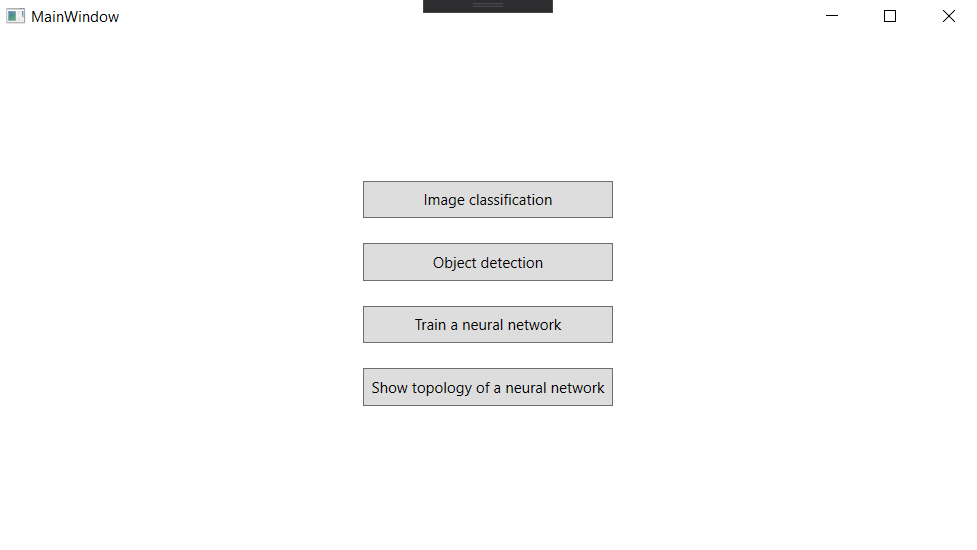
\includegraphics[width=\textwidth]{MainPageGUI}
\caption{Main page of our software}
\end{figure}
\begin{figure}[htb!]\centering
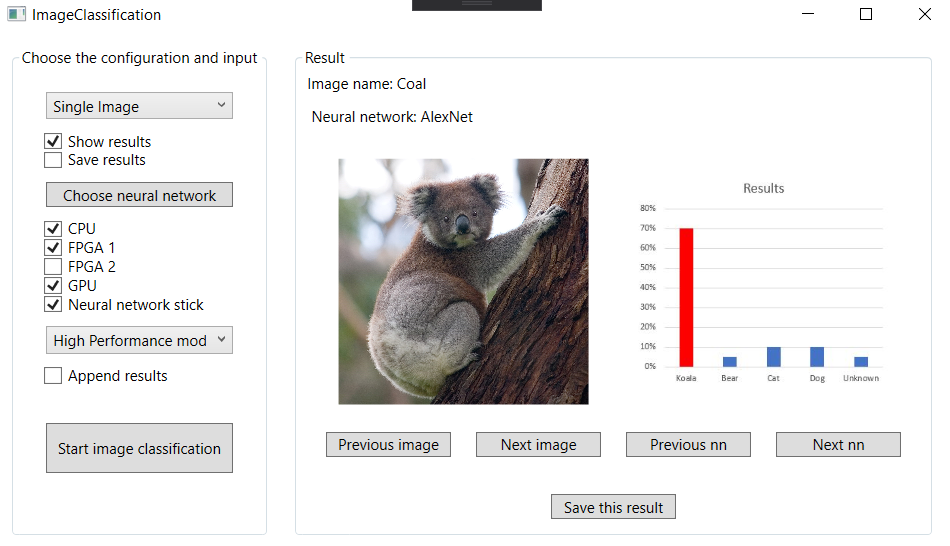
\includegraphics[width=\textwidth]{ImageClassificationGUI}
\caption{Image classification page of our software}
\end{figure}
\begin{figure}[htb!]\centering
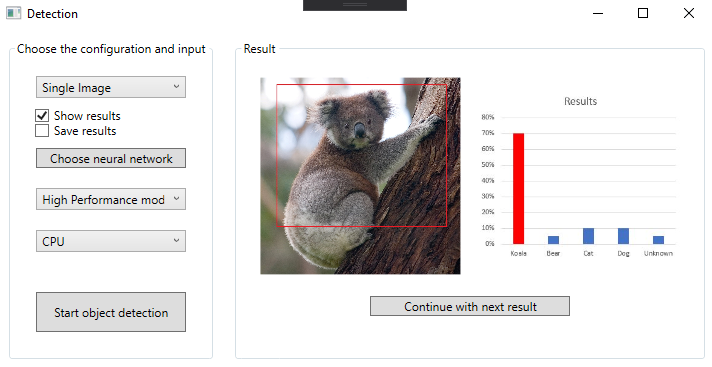
\includegraphics[width=\textwidth]{DetectionGUI}
\caption{Object detection page of our software}
\end{figure}
\begin{figure}[htb!]\centering
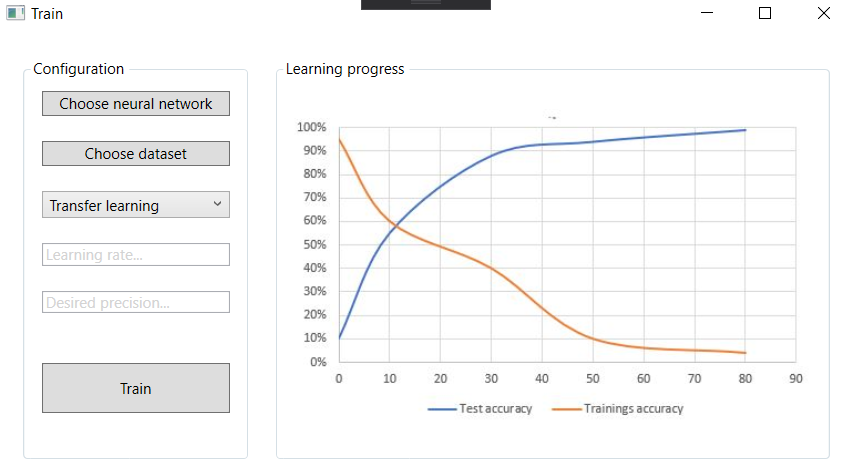
\includegraphics[width=\textwidth]{TrainGUI}
\caption{Training page of our software}
\end{figure}
\begin{figure}[htb!]
\centering
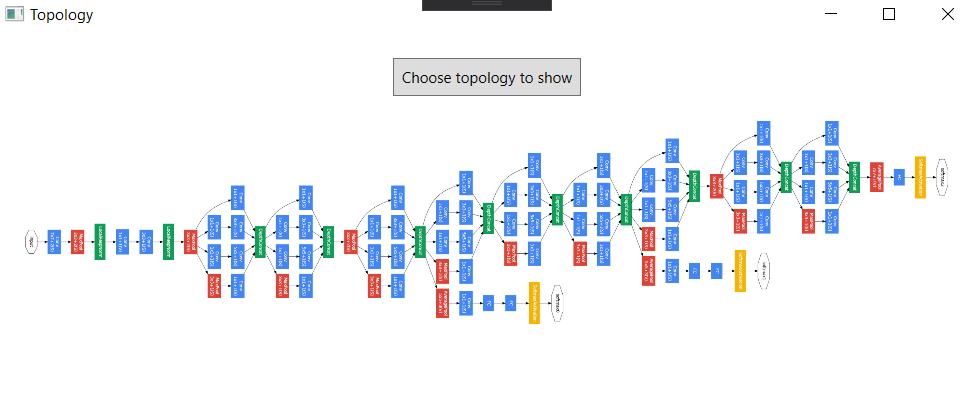
\includegraphics[width=\textwidth]{TopoGUI}
\caption{Page which shows the topology of a selected NN of our software}
\end{figure}
\newpage
\printnoidxglossaries

\end{document}
